\documentclass[t, 11pt]{beamer}
\pdfmapfile{+sansmathaccent.map}
%%% Работа с русским языком
\usepackage{cmap}				
\usepackage{mathtext} 				
\usepackage[T2A]{fontenc}		
\usepackage[utf8]{inputenc}			
\usepackage[english,russian]{babel}	

\usetheme{Ilmenau}
\usecolortheme{lily} % Цветовая схема



%%% Работа с картинками
\usepackage{graphicx}

\usepackage{csquotes}

\hypersetup{				
	colorlinks=true,       	
	linkcolor=blue,          
	citecolor=blue,       
	filecolor=magenta,      
	urlcolor=magenta           
}


\title{Sentiment analysis}
\subtitle{opinion minig}
%\author{Чувакин Сергей}
\date{2.12}
%\institute[<<Анализ больших данных в бизнесе, экономике и обществе>>]{<<Высшая школа экономики>>}
\institute{<<Высшая школа экономики>>}
\begin{document}
	\frame[plain]{\titlepage}
%	\section{Outline}
%	
%	\begin{frame}
%		\frametitle{\insertsection} 
%		\begin{block} {}
%			 
%			\hyperlink{l1}{\beamerbutton{Language models}}
%		\end{block}
%			\begin{block}{}
%		\hyperlink{l2}{\beamerbutton{Probabalistic}}
%		\end{block}
%				\begin{block}{}
%		\hyperlink{l2}{\beamerbutton{Perplexity}}
%		\end{block}
%	\end{frame}
%	

\subsection{Sentiment analysis}
\begin{frame}
	\frametitle{\insertsection}
	\frametitle{\insertsubsection}  
	Sentiment analysis is the automated process of analyzing text data and classifying opinions as negative, positive or neutral
\end{frame}


\begin{frame}
	\frametitle{\insertsection}
	\frametitle{\insertsubsection}  
	Extensions:
	\begin{itemize}
		\item Polarity: if the speaker express a positive or negative opinion
		\item Subject: the thing that is being talked about
		\item Opinion holder: the person, or entity that expresses the opinion.
	\end{itemize}
\end{frame}


\begin{frame}
	\frametitle{\insertsection}
	\frametitle{\insertsubsection} 
	Levels: 
	\begin{itemize}
	\item Document level.
	\item Sentence level .
	\item Sub-sentence level.
\end{itemize}
\end{frame}

\begin{frame}
	\frametitle{\insertsection}
	\frametitle{\insertsubsection}  
	Fine-grained approach: 
	\begin{itemize}
	\item Very positive
	\item Positive
	\item Neutral
	\item Negative
	\item Very negative
\end{itemize}
\end{frame}



\begin{frame}
	\frametitle{\insertsection}
	\frametitle{\insertsubsection}  
	Technical approaches:
\begin{itemize}
	\item Rule-based (lexicon based)
	\item Automatic
	\item Hybrid
	\end{itemize}
\end{frame}

\begin{frame}
	\frametitle{\insertsection}
	\frametitle{\insertsubsection}  
	Rule-based.
	
	N-Negative \ N-Positive words
	
\end{frame}



\subsection{ML}
\begin{frame}
	\frametitle{\insertsection}
	\frametitle{\insertsubsection}  
	After feature extraction: 
	\begin{itemize}
		\item Naïve Bayes
		\item Linear Regression
		\item SVM  
		\item DL
	\end{itemize}
	 
\end{frame}




\subsection{ML}
\begin{frame}
	\frametitle{\insertsection}
	\frametitle{\insertsubsection}  
Challenges
	\begin{itemize}
		\item Tone
		\item Context and Polarity
		\item Comparisons  
		\item Emojis
		\item Defining Neutral	
	\end{itemize}

<<This product is second to none.>>

<<This is better than old tools.>>

<<This is better than nothing.>>
	
\end{frame}





%	\begin{frame}
%	\frametitle{\insertsection}
%	\frametitle{\insertsubsection}  
%	Синонимы кватификаторов 
%	\begin{center}
%		\begin{table}[]
%			\begin{tabular}{c|c|c}
%				\hline
%				Синоним &Расшифровка &Квантификатор \\
%				\hline
%		+ & 1 и более раз &\{1,\}   \\
%		* & 0 и более раз &\{0,\}   \\
%
%		? &  0 или 1 раз& \{0,1\}  \\
%  
%			\end{tabular}
%		\end{table}
%	\end{center}
%\end{frame}

%\begin{frame}
%	\frametitle{\insertsection}
%	\frametitle{\insertsubsection}  
%	Чтобы убрать жаность необходимо добавить ?
%	
%	\vspace{0.5cm}
%	
%	Строка на вход  <<( dfghvb ) sdvsd ( sdcvkjnh ) sdvsd ( dkjhvgr ) sdvfv.>>
%	
%	\vspace{0.5cm}
%	
%	шаблон: r"$\backslash$(.+?$\backslash$)"
%	
%	\vspace{0.5cm}
%	
%	на выходе: ['dfghvb', 'sdcvkjnh', 'dkjhvgr']
%	
%\end{frame}



%	\begin{frame}
%	\frametitle{\insertsection}
%	\frametitle{\insertsubsection}
%	
%	
%	\vspace{1cm}
%	\includegraphics[width=0.9\linewidth]{page2.png}
%	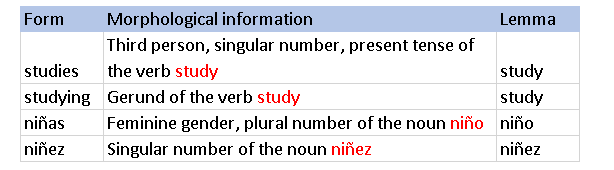
\includegraphics[width=0.7\linewidth]{lem.png}
%\end{frame}
\end{document}